\chapter{Controller Design}\label{ch:ControllerDesign}
\section{Controller Structure}
\begin{figure}[ht]
    \centering
    \includegraphics[scale=0.45]{img/controllerStructure.png}
    \caption{Overall controller structure of the VSR under unbalanced grid voltage conditions}
    \label{fig:controllerStructure}
\end{figure}
\section{Current Controller}
The internal PI current controller's are popular in the industrial application for the reasons,
that it is easy to implement and has low computational burden
which is a nesseccity for high bandwidth systems like the active rectifier.\par
The mathematical model developed in equation [\ref{eq:state_space_dq_positive}] 
and [\ref{eq:state_space_dq_negative}] describes the dynamics of the system
and serves as the basis for the d and q current controller design. The $\omega L$ 
term presents a coupling effect between the d and q axes, which must
be considered in the controller design.\par
\begin{figure}[ht]
\centering
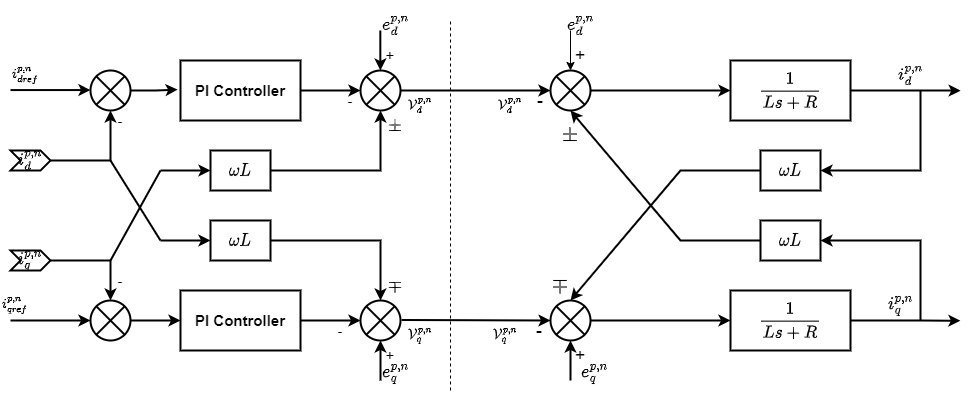
\includegraphics[scale = 0.5]{img/decoupledController.png}
\caption{Diagram of decoupled current controller}
\label{fig:decoupledController}
\end{figure}
\subsection{Cross Coupling cancellation}
To design a PI controller for the current control loop, the cross coupling terms must be cancelled out.
This is done by adding a feed forward term to the controller as shown in figure [\ref{fig:decoupledController}].
The control variable $\mathcal{V}_{d}$ and $\mathcal{V}_{q}$ are defined as in equations[\ref{eq:control_positive}]
and [\ref{eq:control_negative}], the system can be decoupled and the cross coupling terms are cancelled out.
\begin{equation}
    \begin{split}
        \mathcal{V}_{d}^{p}    &= -\mathcal{U}_{d}^{p} + e_{d}^{p} + \omega L i_{q}^{p} \\
        \mathcal{V}_{q}^{p}    &= -\mathcal{U}_{q}^{p} + e_{q}^{p} - \omega L i_{d}^{p}
    \end{split}
    \label{eq:control_positive}
\end{equation}
\begin{equation}
    \begin{split}
        \mathcal{V}_{d}^{n}    &= -\mathcal{U}_{d}^{n} + e_{d}^{n} - \omega L i_{q}^{n} \\
        \mathcal{V}_{q}^{n}    &= -\mathcal{U}_{q}^{n} + e_{q}^{n} + \omega L i_{d}^{n}
    \end{split}
    \label{eq:control_negative}
\end{equation}
where $\mathcal{U}_{d}$ and $\mathcal{U}_{q}$ are the new control variables for the decoupled system. 
The system can now be represented as in equations [\ref{eq:decoupled_positive}] and [\ref{eq:decoupled_negative}]:
\begin{equation}
    \begin{split}
        L \frac{di_{d}^{p}}{dt} &= -R i_{d}^{p} +  \mathcal{U}_{d}^{p}\\
        L \frac{di_{q}^{p}}{dt} &= -R i_{q}^{p} +  \mathcal{U}_{q}^{p}
    \end{split}
    \label{eq:decoupled_positive}
\end{equation}
\begin{equation}
    \begin{split}
        L \frac{di_{d}^{n}}{dt} &= -R i_{d}^{n} +  \mathcal{U}_{d}^{n}\\
        L \frac{di_{q}^{n}}{dt} &= -R i_{q}^{n} +  \mathcal{U}_{q}^{n}
    \end{split}
    \label{eq:decoupled_negative}
\end{equation}
The Laplace transform of the decoupled system $G(s)$ is given in equations [\ref{eq:decoupled_laplace}]:
\begin{equation}
    G(s) = \frac{I(s)}{U(s)} = \frac{1}{Ls + R}
    \label{eq:decoupled_laplace}
\end{equation}
\subsection{PI Current Controller Design}
The PI current controller is designed based on decoupled differential equation in equation [\ref{eq:decoupled_laplace}].
Let's define an auxiliary control variable $\mathcal{U}_{d}$ and $\mathcal{U}_{q}$ as in equations 
[\ref{eq:aux_control_positive}] and [\ref{eq:aux_control_negative}]:
\begin{equation}
    \begin{split}
        \mathcal{U}_{d}^{p}    &= (i_{dref}^{p} - i_{d}^{p}) (k_{p} + \frac{k_{i}}{s})\\
        \mathcal{U}_{q}^{p}    &= (i_{qref}^{p} - i_{q}^{p}) (k_{p} + \frac{k_{i}}{s})
    \end{split}
    \label{eq:aux_control_positive}
\end{equation}
\begin{equation}
    \begin{split}
        \mathcal{U}_{d}^{n}    &= (i_{dref}^{n} - i_{d}^{n}) (k_{p} + \frac{k_{i}}{s}) \\
        \mathcal{U}_{q}^{n}    &= (i_{qref}^{n} - i_{q}^{n}) (k_{p} + \frac{k_{i}}{s})
    \end{split}
    \label{eq:aux_control_negative}
\end{equation}
where $k_{p}$ and $k_{i}$ are the proportional and integral gains of the PI controller respectively.\par
The closed loop transfer function of the system can be derived as in equation [\ref{eq:closed_loop_transfer_function}]:
\begin{equation}
    \frac{I(s)}{I_{ref}(s)} = \frac{(k_{p} + \frac{k_{i}}{s}) \frac{1}{Ls + R}}{1 + (k_{p} + \frac{k_{i}}{s}) \frac{1}{Ls + R}} 
    = \frac{k_{p} s + k_{i}}{L s^{2} + (R + k_{p}) s + k_{i}}
    \label{eq:closed_loop_transfer_function}
\end{equation}
To achieve a desired closed loop performance, among the various tuning methods, Internal Model Control (IMC)
has been used for PI controller tuning for past decades in systems where an approximate model is available.
This technique allows for adequate tracking and excels in disturbance rejection\cite{Shamsuzzoha2012, artIMCPIDShah}.
The imperfect model should be incorporated as part of the controller design using an explicit model of the plant 
\cite{Shamsuzzoha2012}. This tuning provides robustness to the controller, with the control loop remaining stable
even if the parameters change substantially from those used for tuning. This is an interesting feature for the real
implementation of the VSC.\par
The primary disadvantage of IMC PI tuning is that it sets the PI integral part to be equal to
the process time constant. Therefore, if the process had a long time constant, the controller
would have an equally long integral time, resulting in slow recovery from process disturbances.
However, for the VSC application, the process time constant is fast enough that it does not
interfere with the desired controller behavior.\par
The IMC tuning rules for a first order system $P(s)$ is given in equations [\ref{eq:IMC_tuning_kp}] and [\ref{eq:IMC_tuning_ki}]:
\begin{equation}
    P(s) = \frac{K}{\tau s + 1}
    \label{eq:first_order_system}
\end{equation}
\begin{equation}
    k_{p} = \frac{\tau}{K \tau_c}
    \label{eq:IMC_tuning_kp}
\end{equation}
\begin{equation}
    k_{i} = \frac{k_p}{\tau}
    \label{eq:IMC_tuning_ki}
\end{equation}
where $\tau_c$ is the desired closed loop time constant and $\tau$ is the process time constant.\par
A smaller $\tau_c$ results in a faster response but reduces the robustness of the controller.
Conversely, a larger $\tau_c$ increases robustness but slows down the response.\par
Thus, to design the PI current controller using IMC tuning rules, the process gain $K$ and time constant $\tau$
must be identified from the decoupled transfer function in equation [\ref{eq:decoupled_laplace}]:
\begin{equation}
    P(s) = G(s) = \frac{K}{\tau s + 1}= \frac{\frac{1}{R}}{\frac{L}{R}s + 1}
    \label{eq:transfer_function_identification}
\end{equation}
From equation [\ref{eq:transfer_function_identification}], the process gain $K$ and time constant $\tau$ are identified as:
\begin{equation}
    K = \frac{1}{R}, \quad \tau = \frac{L}{R}
    \label{eq:process_parameters}
\end{equation}
From equations [\ref{eq:IMC_tuning_kp}], [\ref{eq:IMC_tuning_ki}] and [\ref{eq:process_parameters}], the PI controller gains
can be derived as:
\begin{equation}
    k_{p} = \frac{L}{\tau_c}
    \label{eq:final_kp}
\end{equation}
\begin{equation}
    k_{i} = \frac{R}{\tau_c}
    \label{eq:final_ki}
\end{equation}
Once the PI controller gains are determined, they can be implemented in the closed loop transfer function 
[\ref{eq:final_closed_loop_transfer_function}] to analyze the system performance.obtained from equation 
[\ref{eq:closed_loop_transfer_function}] to analyze the system performance.
\begin{equation}
    \begin{split}
    \frac{I(s)}{I_{ref}(s)} &=  \frac{(k_{p} + \frac{k_{i}}{s}) \frac{1}{Ls + R}}{1 + (k_{p} + \frac{k_{i}}{s}) \frac{1}{Ls + R}} \\
    \frac{I(s)}{I_{ref}(s)} &= \frac{1}{\tau_c s + 1}
    \end{split}
    \label{eq:final_closed_loop_transfer_function}
\end{equation}
The bandwidth of the current controller is chosen to be at least ten times smaller than the
switching frequency of the inverter to ensure that the controller can respond quickly enough to
changes in the reference current.
\begin{equation}
    \tau_c = \frac{10}{2 \pi f_{s}}
    \label{eq:time_constant_bandwidth}
\end{equation}
\section{DC Voltage Controller}
The DC voltage controller is designed to regulate the DC link voltage of the VSR to a desired reference value.

\section{Phase Locked Loop (PLL)}
To ensure proper operation of the VSR under unbalanced grid voltage conditions,
a robust phase-locked loop (PLL) is essential for accurate grid voltage phase angle and frequency estimation.
The angle information provided by the PLL is crucial for the transformation of
grid voltages and currents into the synchronous reference frame (dq frame).
The PLL structure used in this work is illustrated in figure [\ref{fig:PLLstructure}].\par
\begin{figure}[ht]
    \centering
    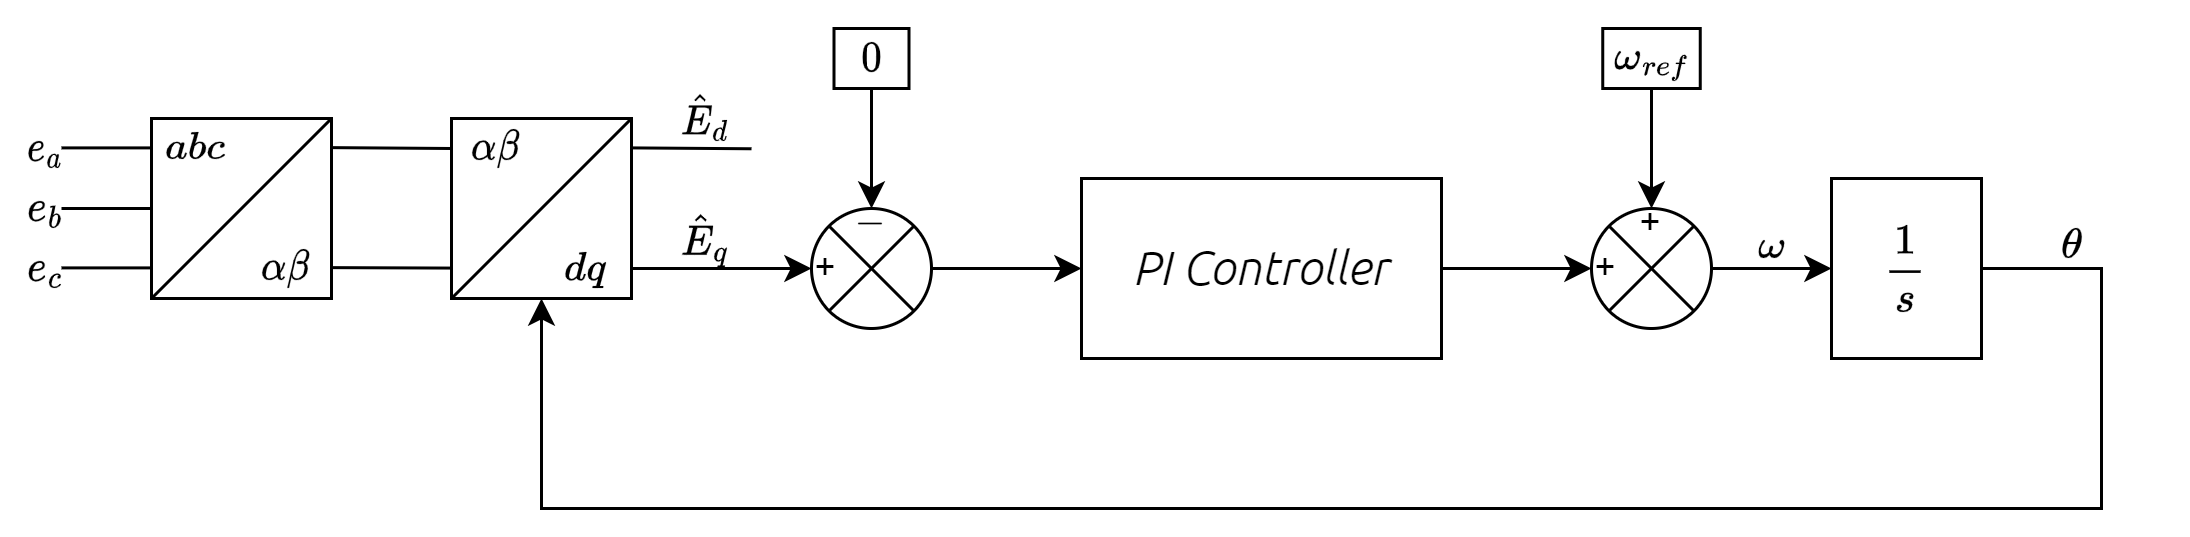
\includegraphics[scale=0.75]{img/PLL_Block_Diagram.png}
    \caption{Block diagram of the PLL structure}
    \label{fig:PLLstructure}
\end{figure}
The PLL takes the three-phase grid voltages as input, which are first transformed into the $\alpha \beta$
stationary reference frame using the Clarke transformation. The $\alpha \beta$ voltages are then converted
into the dq synchronous reference frame using the Park transformation, which requires an initial estimate
of the grid voltage angle $\theta$. The q-axis voltage component $v_{q}$ is used as the error signal for the PLL,
which is processed by a PI controller to adjust the estimated angle $\theta$.\par
The PLL is designed to minimize the q-axis voltage component $v_{q}$, which ideally should be zero when the estimated 
angle $\theta$ matches the actual grid voltage angle. The PI controller in the PLL adjusts the estimated angle based on
the error signal, ensuring that the PLL can track changes in the grid voltage angle and frequency accurately.\par
The PLL is designed to according \cite{PLL7467498, PLLWang2019}
\begin{equation}
    \begin{split}
        \dot{\omega}  &= \gamma_1 \varepsilon\\
        \dot{\theta} &= \omega + \gamma_2 \varepsilon
    \end{split}
    \label{eq: PLL model}
\end{equation}
where $\varepsilon$ is the PLL error signal of $v_q$, $\omega$ is the estimated angular frequency, $\theta$ is the estimated angle,
and $\gamma_1$, $\gamma_2$ are the PLL PI controller gains ($\gamma_1$ is the integral gain, $\gamma_2$ is the proportional gain).\par
The PI controller gains are designed based on the desired PLL bandwidth $\rho$ and $\hat{E}_g$ as shown in equations
[\ref{eq: PLL gain 1}], [\ref{eq: PLL gain 2}] and [\ref{eq: resultant voltage}]:
\begin{equation}
    \gamma_1 = \frac{\rho^2}{\hat{E}_g}
    \label{eq: PLL gain 1}
\end{equation}
\begin{equation}
    \gamma_2 = 2 \frac{\rho}{\hat{E}_g}
    \label{eq: PLL gain 2}
\end{equation}
\begin{equation}
    \hat{E}_g = \sqrt{\hat{E}_d^2 + \hat{E}_q^2}
    \label{eq: resultant voltage}
\end{equation}
\begin{figure}[ht!]
    \centering
    % First row of images
    \subfloat[Balanced voltage input in abc frame]{
        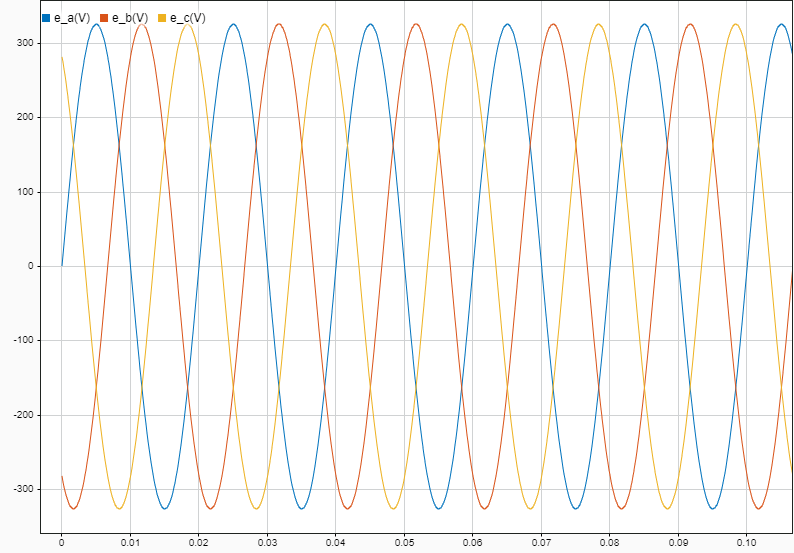
\includegraphics[width=0.45\linewidth]{img/PLL_balanced_voltage_abc.png}
        \label{subfig:a voltage input }
    }
    \hfill
    \subfloat[Balanced voltage input in $\alpha\beta$ frame]{
        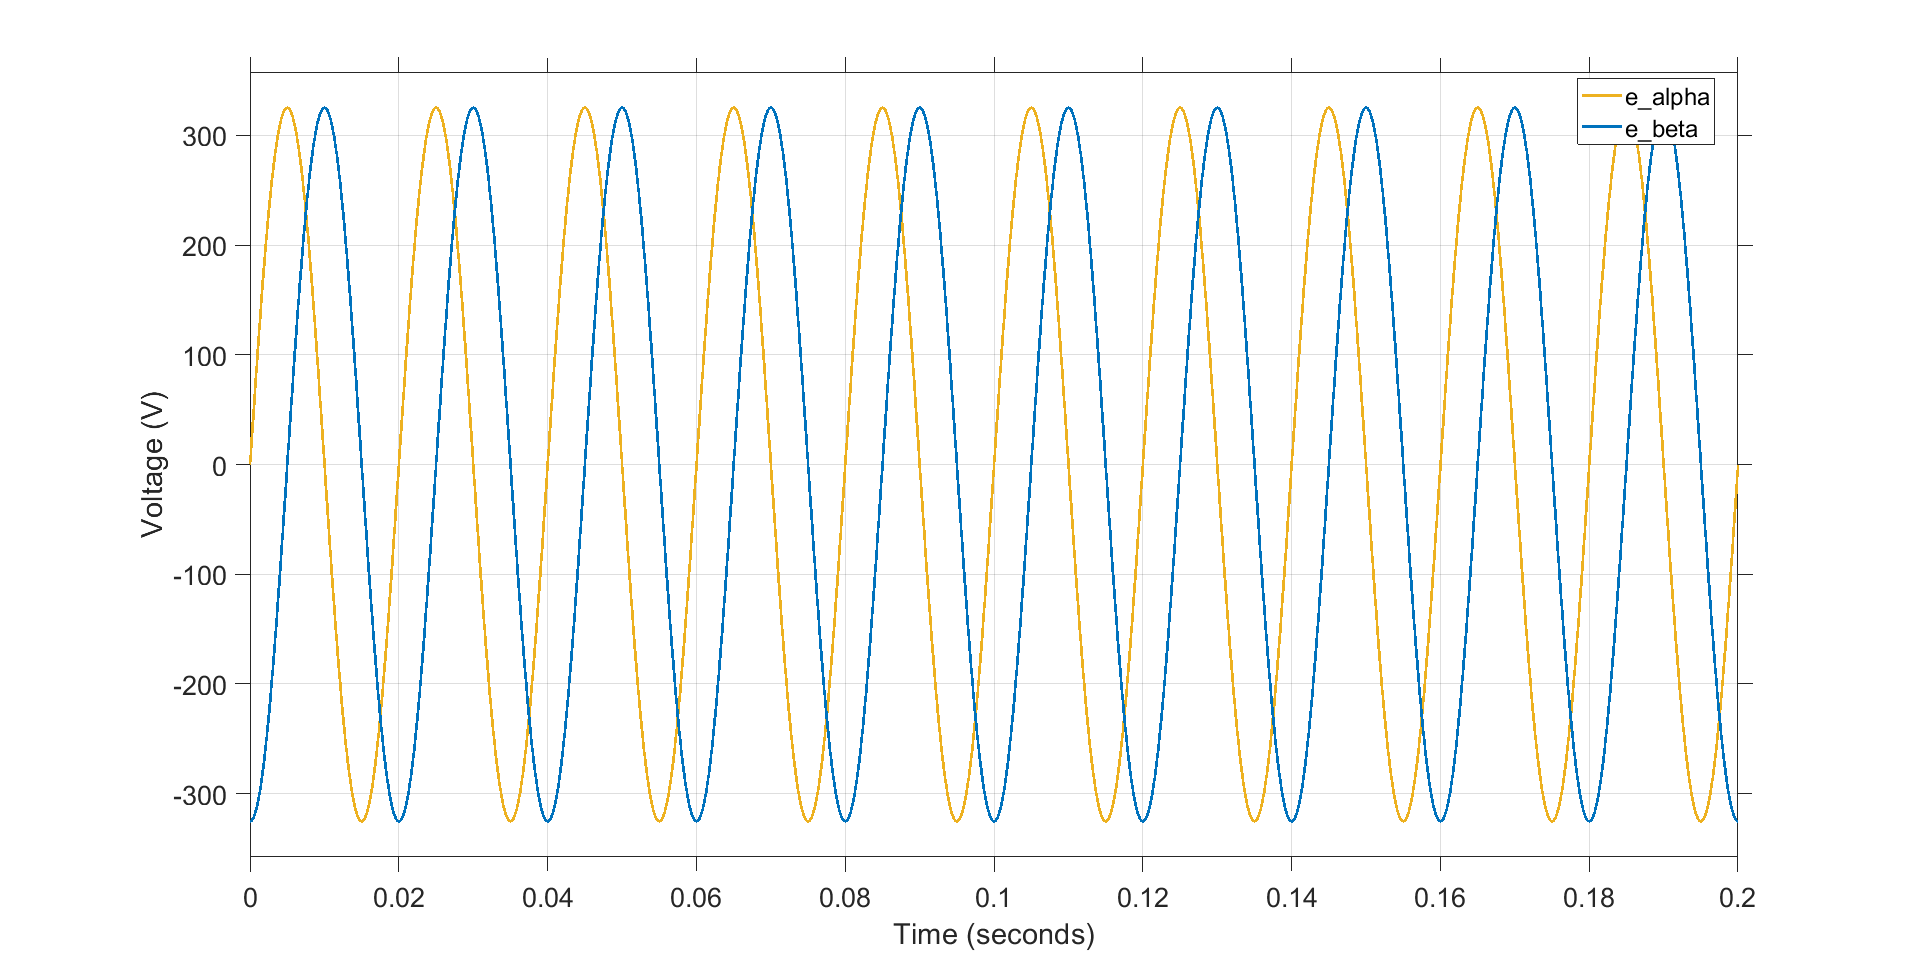
\includegraphics[width=0.45\linewidth]{img/PLL_balanced_voltage_alphabeta.png}
        \label{subfig:b voltage input alphabeta }
    }\\
    \subfloat[Balanced voltage input in dq frame]{
        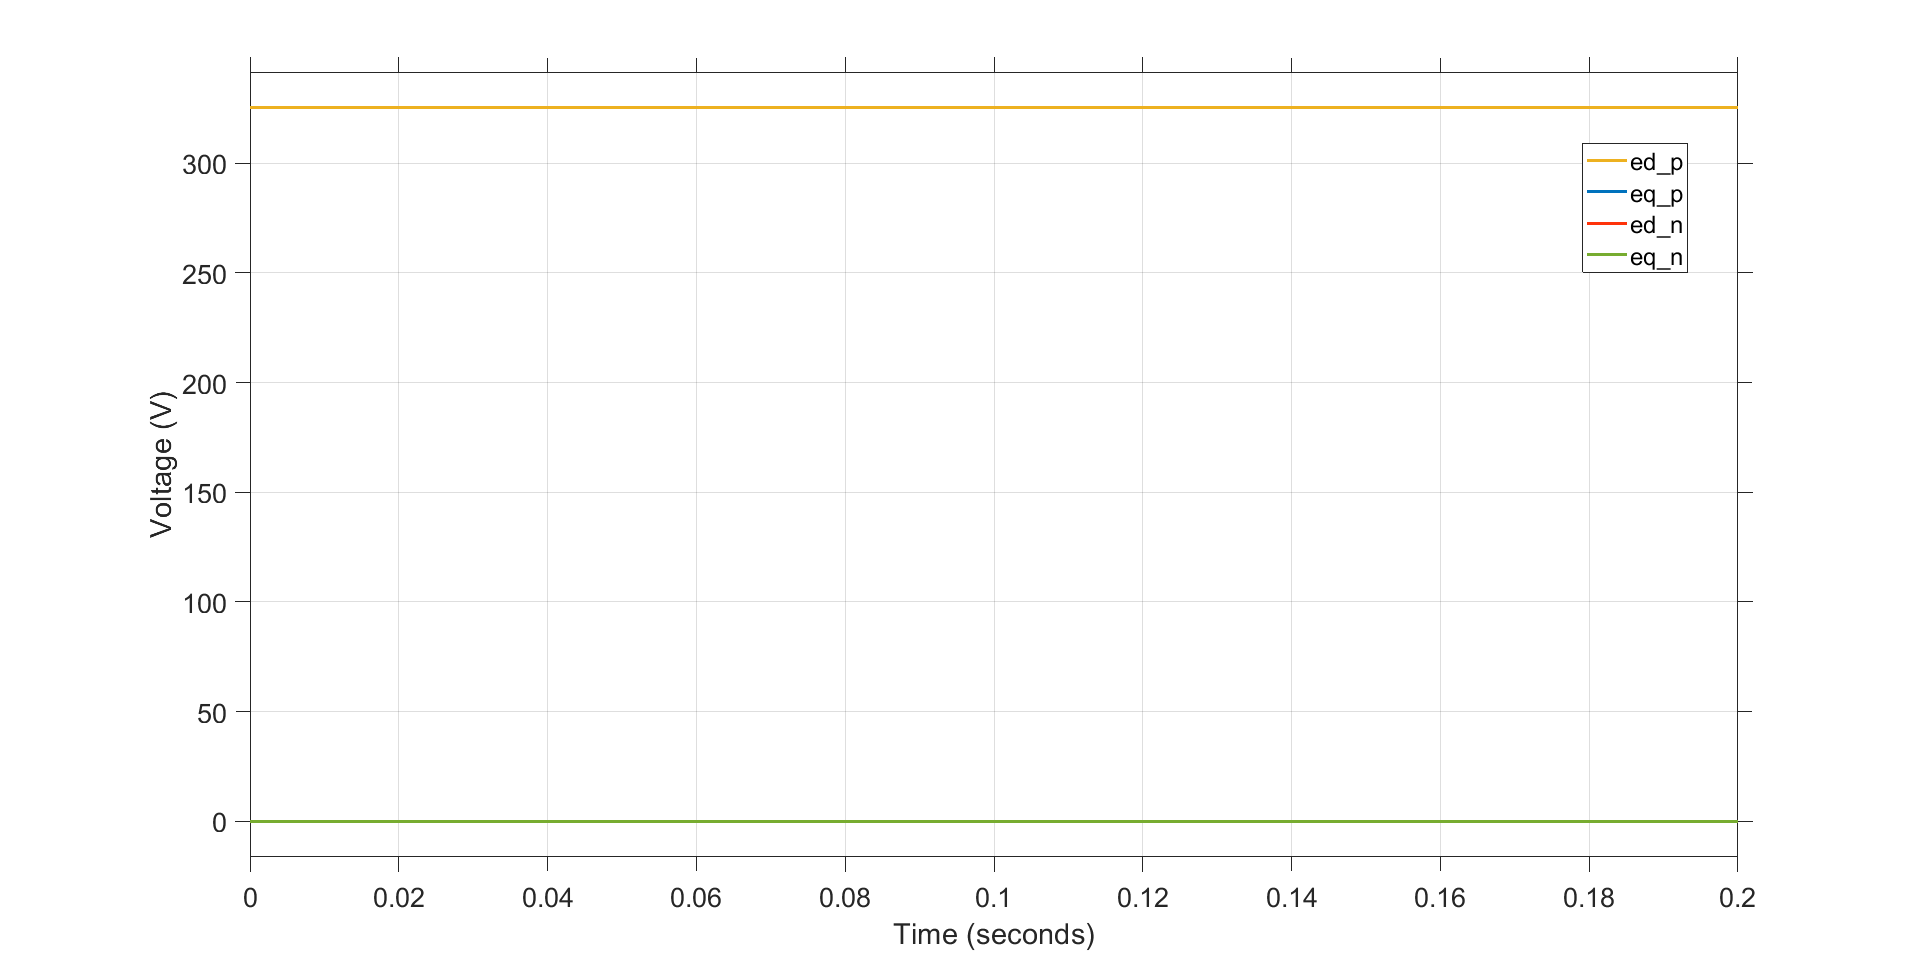
\includegraphics[width=0.45\linewidth]{img/PLL_balanced_voltage_dq.png}
        \label{subfig:c voltage input dq}
    }
    \hfill
    \subfloat[PLL Angle estimation]{
        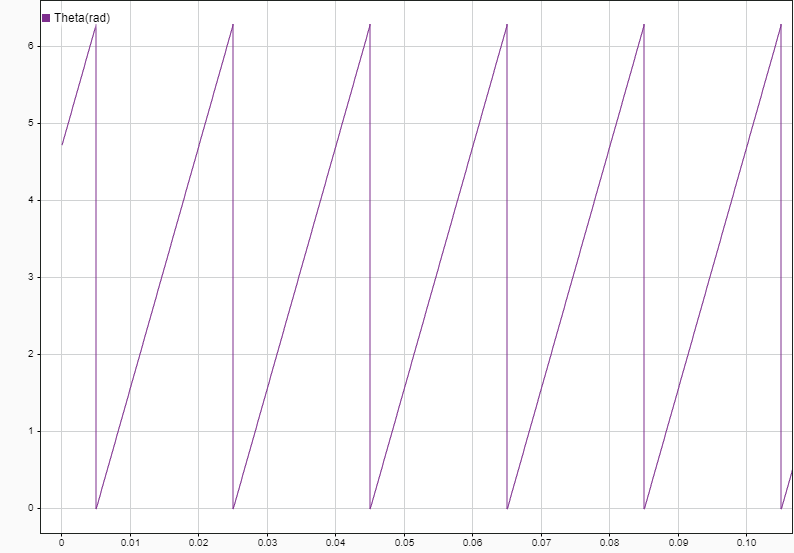
\includegraphics[width=0.45\linewidth]{img/PLL_balanced_theta.png}
        \label{subfig:d angle estimation }
    }
    \caption{Overall caption for the 2x2 grid of images.}
    \label{fig:balanced_PLL}
\end{figure}

\begin{figure}[ht!]
    \centering
    % First row of images
    \subfloat[Unbalanced voltage input in abc frame]{
        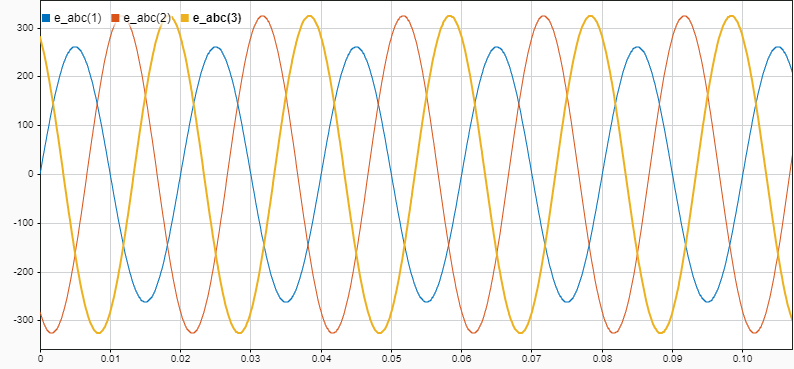
\includegraphics[width=0.45\linewidth]{img/PLL_unbalanced_voltage_abc.png}
        \label{subfig:a voltage input abc}
    }
    \hfill
    \subfloat[positive sequence voltage in abc frame]{
        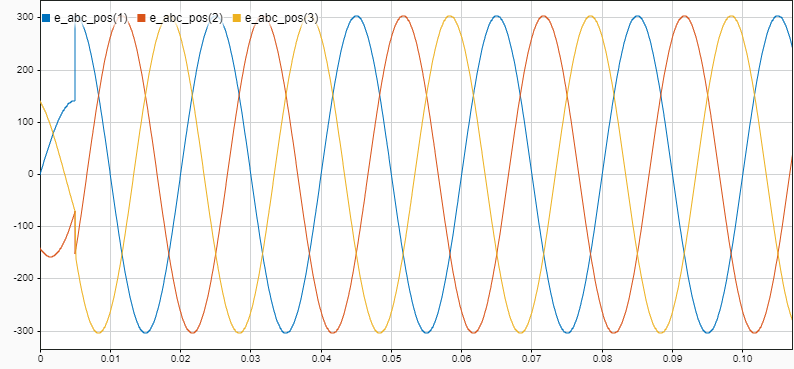
\includegraphics[width=0.45\linewidth]{img/PLL_unbalanced_voltage_abc_pos.png}
        \label{subfig:b voltage input positive abc }
    }\\
    \subfloat[negative sequence voltage in abc frame]{
        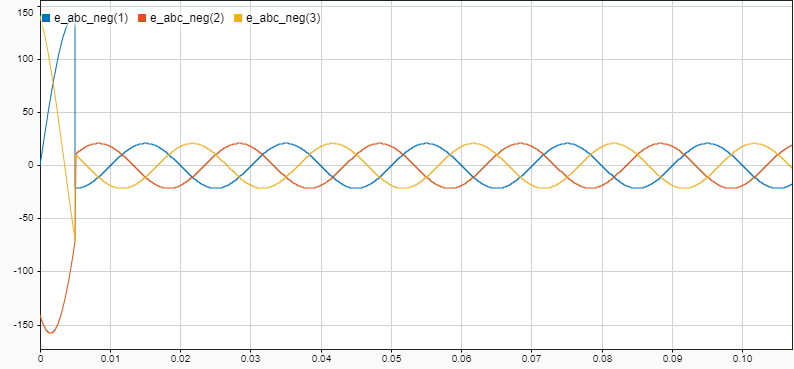
\includegraphics[width=0.45\linewidth]{img/PLL_unbalanced_voltage_abc_neg.png}
        \label{subfig:c voltage input negative abc}
    }
    \hfill
    \subfloat[positive sequence voltage in $\alpha\beta$ frame]{
        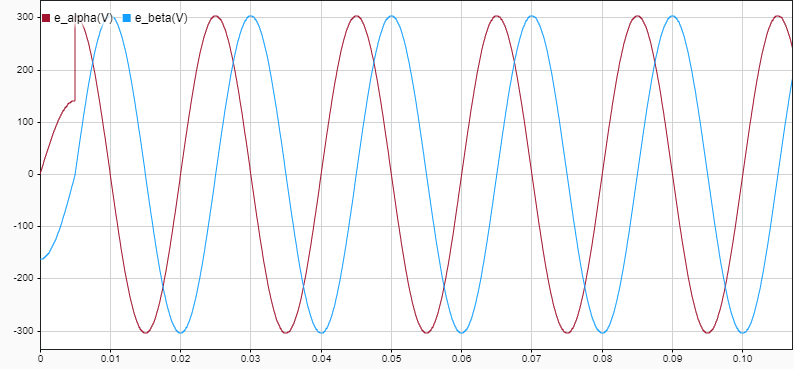
\includegraphics[width=0.45\linewidth]{img/PLL_unbalanced_voltage_alphabeta_pos.png}
        \label{subfig:d voltage input positive alphabeta}
    }\\
    \subfloat[positive sequence voltage in dq frame]{
        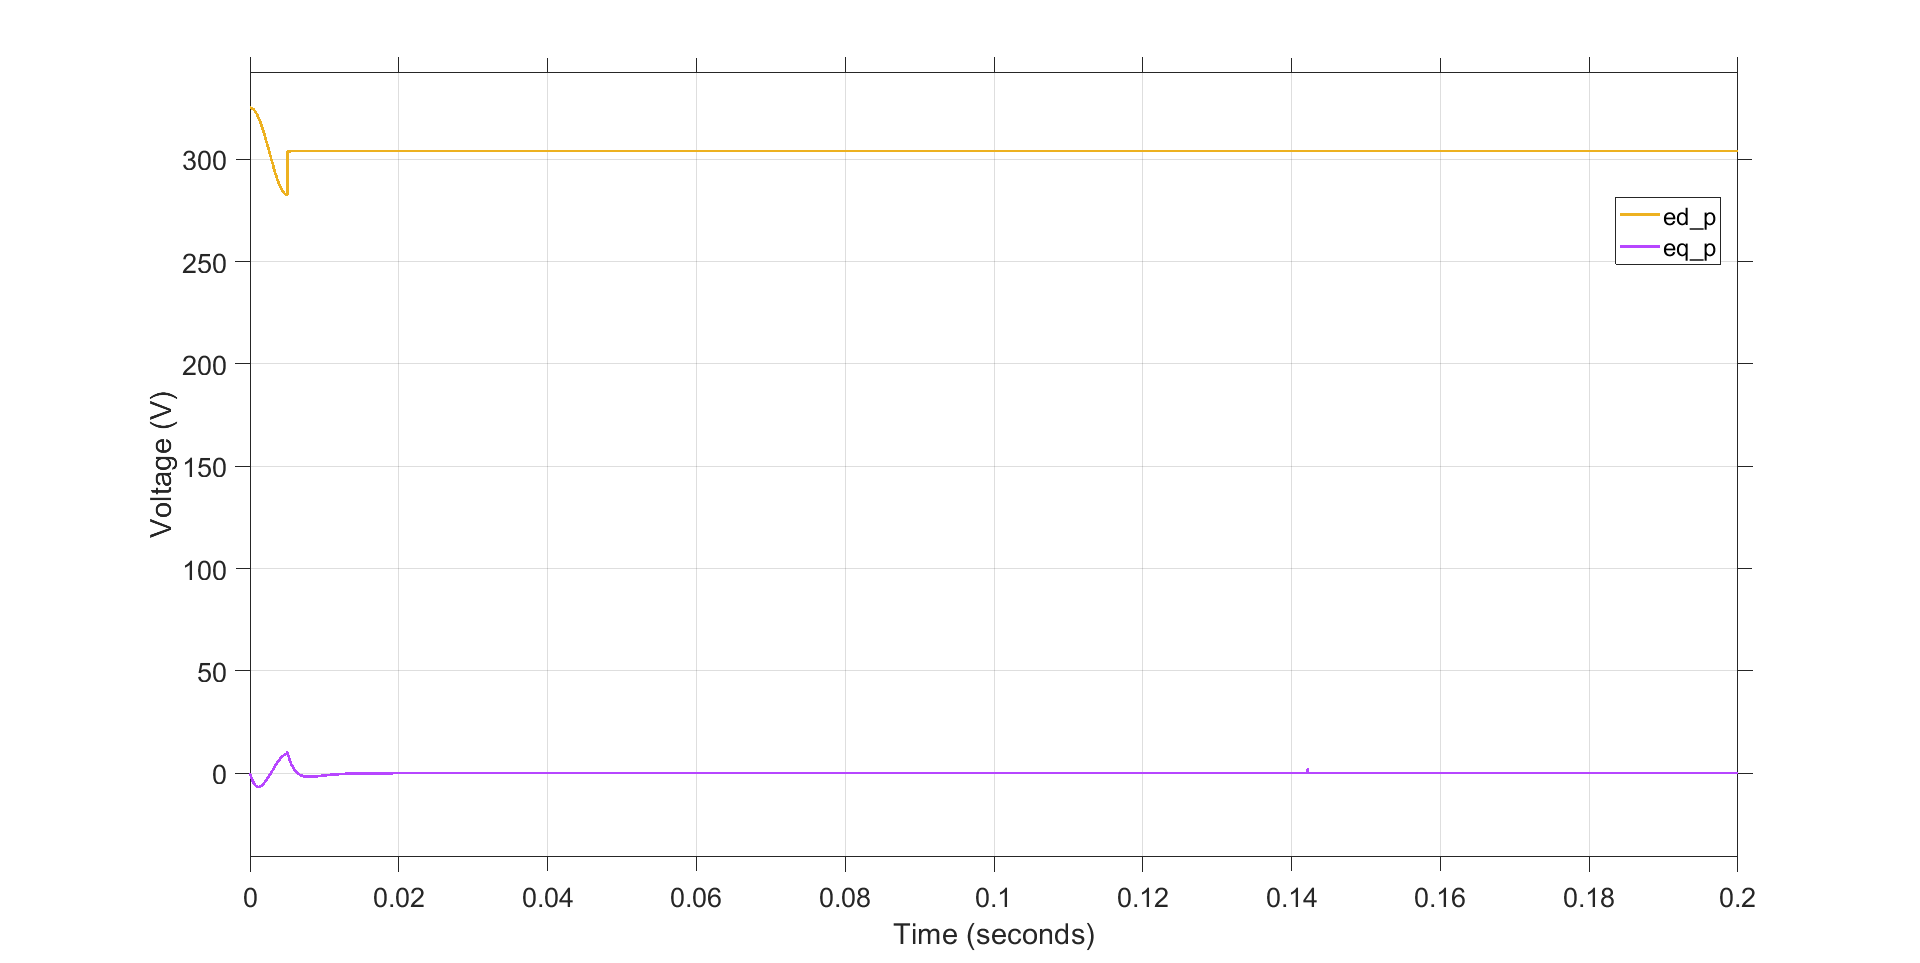
\includegraphics[width=0.45\linewidth]{img/PLL_unbalanced_voltage_dq_pos.png}
        \label{subfig:e voltage input positive dq}
    }
    \hfill
    \subfloat[PLL Angle estimation]{
        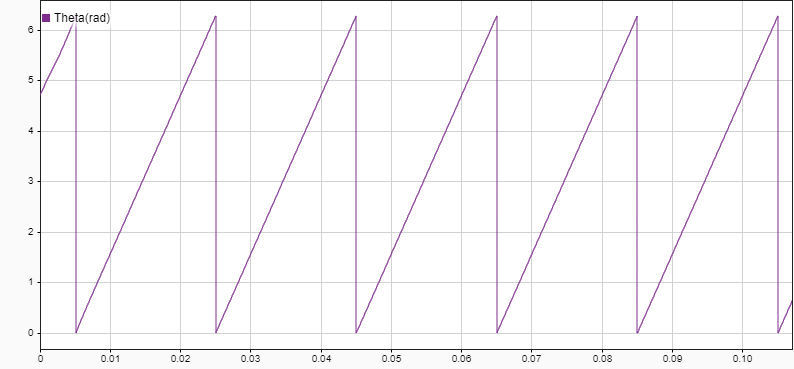
\includegraphics[width=0.45\linewidth]{img/PLL_unbalanced_theta.png}
        \label{subfig:f angle estimation }
    }
    \caption{Overall caption for the 3x2 grid of images.}
    \label{fig:unbalanced_PLL}
\end{figure}
